\chapter{Review and Summary}

The aim of this set of studies was to identify how attributes of network architecture allow for the cognitive flexibility required for skilled reading. We combined inferences from several different methodological approaches, including resting-state network analysis, task-based activation analyses, and the combination of the two.  

Here, we asked how network architecture could inform our understanding of cognitive flexibility, especially in an integrative model such as reading. Reading utilizes a variety of cognitive skills whose neural substrates are distributed throughout the brain. Graph theory has enabled analysis...
Important properties... modules... hubs...
Individual differences not well understood...
Development through interactive specialization...

In Study 1, we analyzed resting-state network architecture in  fourth grade readers. We established a set of connectome-forming methods and settled on a set of descriptive metrics including modularity, participation coefficient and path length. Next, we compared individual differences in these attributes to reading skill. We found that better readers had greater global network modularity but reduced modularity in the auditory and cingulo-opercular RSNs, suggesting that this segregated network architecture is important for functioning but that literacy acquisition may impact the composition of specific networks. 

We next sought to describe how network architecture, and its relationship to reading, changes \textit{during} reading. In Study 2, we observed that reading comprehension decreased global modularity, especially in the visual, dorsal attention and default mode networks. Overall, it increased measures of integration between a wide-variety of RSNs, including sensory and attention systems. Furthermore, the positive relationship between reading skill and global modularity persisted during comprehension, suggesting that the maintenance of each module across tasks is an important attribute of an efficient connectome. 

Does that mean that \textit{more} similarity between task-evoked network architectures is more indicative of an efficient organization? If so, do flexible hubs provide a way in which RSNs can increase inter-connectivity without disrupting RSN integrity?  To answer these questions, Study 3 compared two related but different processes - reading and listening. We found that there was a common core of areas activated in the two network states, as well as a common network backbone. In fact, better readers had a greater degree of similarity between the two language conditions, suggesting that the two networks merge in more skilled readers. We then calculated network flexibility across many different architectures, including simple attention tasks and rest and found that the listening-to-reading similarity was not unique to language, but inherent to the individual: participants were generally more similar to themselves in different tasks than to others in the same task.

Finally, we investigated the effects of development on modularity and network organization. In Chapter 5, we replicated these findings with an independent task and also described the findings across development. We found that similarity between listening and reading - and indeed, all tasks -- changed over time. ...

\begin{table}[t]
	\renewcommand{\tabcolsep}{0.2cm}
	\centering
	\begin{tabular}{c|p{10cm}}
\toprule 
Figure & Key Finding \\ 
\midrule 
\ref{fig:ch2-global-glm-covariates-thresh} & Global modularity was the graph theory measurement most predictive of reading skill. \\ 
 \ref{fig:ch2-rsn-node-modularity-corr} & Modularity in the auditory and cingulo-opercular networks was anti-correlated with reading skill.	\\ 
\ref{fig:ch3-reading-connectome-activations} & Reading comprehension induces system-level increases in the ventral attention, visual, somatomotor (mouth) and default mode networks.	 \\ 
\ref{fig:ch3-comprehension-reorganization}  & Reading is especially characterized by decreased connectivity \textit{within} sensory, dorsal attention and default mode and increased connectivity \textit{between} many different RSNs.  \\ 
\ref{fig:ch3-modularity-reading-by-condition}  & The positive relationship between network modularity and reading persists during reading comprehension.  \\ 
\ref{fig:ch4-modality-graph-theory}  & Reading comprehension requires more more integration across networks than listening. \\ 
\ref{fig:ch4-modality-similarity-to-reading} & Better readers have greater similarity between their listening and reading networks.
\bottomrule 
\end{tabular}
	\caption[Key findings in Studies 1 through 4.]{Key findings in Studies 1 through 4.}
	\label{table:ch6-key-findings}
\end{table}

These studies illustrate how a connectomics approach to reading illuminates -- not displaces -- previous neuroimaging research, much of which focused on localizing specific cognitive processes. We have used reading skill as a model for understanding how individual differences in network architecture form a basis for individual differences in cognitive processing. Through this systematic approach to describing these samples, we have made a contribution to our understanding brain modularity as it realtes to reading skill. However, there is much left to be investigated. Below, we outline a few of these directions.

\section{Individualized parcellations}

A caveat with connectomics analyses, including those presented here, are that results for the modularity analyses are often based on RSN parcellations from previous literature (e.g. \citep{Power2011}) and are applied indiscriminately across the entire group. This allows for a common reference partition and more interpretable results, but it neglects the fact that there may be important differences between individuals in the optimal community partition for an individual. Even within a given method, there can be a very large number of alternative community parcellations that may differ from the maximum in only a very slight way \citep{Good2010}. Community-agnostic measurements such as the intersection of the union, which we employed in the present analyses, or consensus-based clustering, such as that used in \citep{Power2011}, can address some of these concerns, but is still essentially limited in its ability to allow variability of possible partitions in to the system. 

The problem may be especially acute in the context of development. As we noted in Study 4, as children mature, the pattern of connectivity changes significantly, with modules becoming more segregated and long-range RSNs such as the fronto-parietal network becoming more robustly connected \citep{Cao2016}. In cases where there are actual differences in the architecture, comparison to the same reference partition will result in one group being considered lower modularity when in fact they are more appropriately deemed \textit{different} modularity. One way to address this would be to partition each subject's network individually and investigate changes in connectivity longitudinally. This avoids the problem of the ``group average'' structure and allows for an exploration of changes to the community affiliations at an individual level. 

\section{Multi-modal and multi-scale analysis}

In this dissertation, we have dealt exclusively with whole-brain functional connectivity networks. MRI, however, represents only a narrow sliver of the possible methods for undersanding the network architecture of the brain, and how it differs between individuals. Structural connectivity and covariance... 

\begin{figure}[t]
	\centering
	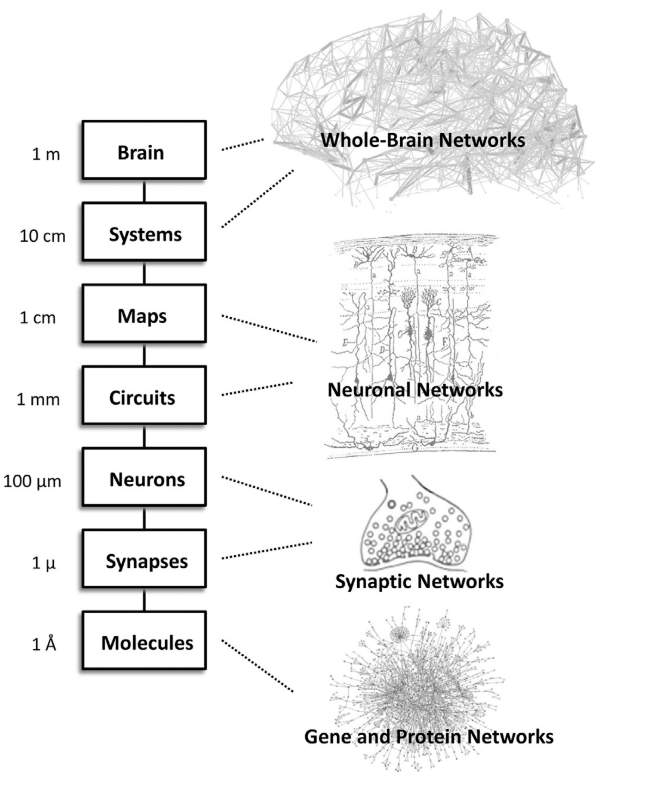
\includegraphics[height=4in]{ch6-multi-scale-connectivity-analysis}
	\caption[Network architecture at multiple scales.]{Network architecture at multiple scales of inquiry. Developing a tight understanding of how measures from the whole-brain network are represented at finer scales is an important future direction. Figure from \citep{Petersen2015}.}
	\label{fig:ch6-multi-scale-connectivity-analysis}
\end{figure}


 (See \citep{Sui2012} for a review of methods connecting different modalities.)

\section{Dynamic modeling of network architecture}

Brain networks are not static, even though they are often modelled as such. Connectivity patterns are constantly shifting, and changes in the configuration of networks across time (so-called dynamic connectivity) have become an increasingly important domain of research in the past several years. Work using sliding time windows have illustrated that during rest modules alternate between time periods of higher and lower levels of integration (e.g. global efficiency) over time \citep{Zalesky2014}. These changes are periodic and can be consistent throughout different parts of the brain \citep{Handwerker2012}. (See Figure \ref{fig:ch6-dynamic-connectivity} for an example.) Modelling this variability across subjects can be a challenge, since subjects states tend not to be locked in time with each other outside of tasks; however, many advances have been had by using wavelets and other techniques \citep{Zalesky2014}. 

\begin{figure}[t]
	\centering
	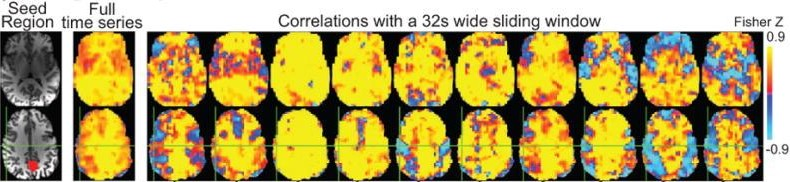
\includegraphics[width=6in]{ch6-dynamic-connectivity}
	\caption[Correlations between brain regions fluctuate over time.]{Correlations between brain regions fluctuate over time. The above figure shows, from left to right: the posterior cingulate seed region; the correlation map created from the seed using a 10 minute time series; correlation maps created over 32s temporal windows. The shorter correlation windows show how functional connectivity changes over time. The authors were able to parse brain regions based on the temporal frequency of these changes in connectivity \citep{Handwerker2012}.}
	\label{fig:ch6-dynamic-connectivity}
\end{figure}

However, answering this question is crucial to understanding our findings of high modularity in better readers. The networks collected were averaged over a relatively long time period -- the course of a few minutes. In that time, there could have been many transitions between low- and high-modularity states. The frequencies at which the brain cycles through these states could be driving the ``average'' global modularity observed in our studies \citep{Fries2005}.

Another major question relates to the effects of task-switching during reading. Previous research demonstrating the flexibility of the fronto-parietal network in cognition used a task with rapid changes in instructions \citep{Cole2013}. The FPN may thus be critical for the initial switching action in connectivity patterns, after which the network becomes more settled. In the context of reading, individuals will spend time in various stages of the comprehension process: at some point extra attention will be paid to the decoding of the text, at others to the semantic processing, at others to the recall and integration of previous information \citep{Spreng2013}. Looking at the variations in activity at key junctures of the reading task would elucidate the roles of individual RSNs such as the FPN in the construction, maintenance and evaluation of the text \citep{Sakai2008}. The answers would help to identify whether the ``flexibility'' of certain RSNs and connections are an attribute of that connection or of the task.

\section{High-resolution parcellations}

One tension present in network analysis is that of resolution: using too coarse of a sampling of the brain and one risks losing important detail; too fine and one risks introducing extra noise and unneeded complexity. In these analyses we used 264 nodes that have been used in a number of other studies (e.g. \citep{Power2013, Cole2014}). These nodes cover a large range of brain systems and functional subdivisions (defined by meta-analytic techniques), and each node is separated by at least 10 mm, meaning there is less redundant information being measured. However, many new methods for segmenting the brain into functional sub-divisions have been released in the intervening years, some of which combine information from multiple modalities and more than a thousand subjects to identify distinct patches of cortex. 

One of the more influential parcellations has been one developed by Glasser and colleagues using Human Connectome Project data \citep{Glasser2016}. This parcellation utilizes changes in cortical architecture, function, structural connectivity, and topography to delineate 180 cortical areas on each hemisphere of the brain. This large number of areas, and the amount of data it is built on, stands in stark contrast to the 52 Brodmann areas which have long formed the standard schema for analysis. 

The challenges limiting the adoption of these advanced methods is the amount and quality of data required (multiple modalities, little-to-no subject motion), as well as the steep learning curve associated with implementing them in practice (many pieces of software, advanced programming techniques, many different file types). However, as more tutorials become available and software becomes more accessible, future research is likely to reap incredible benefit from these more detailed methods \citep{Poldrack2015}.

\section{Final word}

Reading is an astonishing ability which requires the efficient binding of auditory and visual information, and rapid passing of information through several different systems, including attention, executive and semantic systems.  Reading requires flexibility of coordinating between these different systems. If, as John Steinbeck wrote, ``learning to read is probably the most difficult and revolutionary thing that happens to the human brain,'' then we should not be surprised that individuals with a more efficient architecture perform better. 

John Steinbeck stated that, ``Learning to read is probably the most difficult and revolutionary thing that happens to the human brain, and if you don't believe that, watch an illiterate adult try to do it.''


One of the great questions in psychology is, why are we different? What makes one person able to read and another not? We have argued that skilled reading is a concrete model of an integrative cognitive process to determine whether attributes are predictive of individual differences in cognition. There is much yet to learn about individual differences in cognition, but we believe that graph theoreticl analyses can complement traditional universariate and activati analyses. 